%%=============================================================================
%% Proof of concept
%%=============================================================================
\graphicspath{ {./graphics/} }
\chapter{\IfLanguageName{dutch}{Proof of Concept}{Proof of Concept}}%

De volgende stap binnen deze bachelorproef is het uitwerken van de Proof of Concept. Om dit te beantwoorden, wordt de recent verkregen informatie omgezet naar de praktijk. Het doel van de Proof of Concept is om een oplossing te bieden voor het gestelde probleem. Als eerst wordt er stilgestaan bij de gebruikte netwerkopstelling binnen Azure.
Vervolgens komt de gebruikte infrastructuur aan bod. Daarnaast zal er dieper worden ingegaan op Ansible en de bijhorende playbooks, die instaan voor de configuratie van de firewall. Tot slot wordt er gekeken naar de uitwerking van het powershell script, dat instaat voor het uitvoeren van de controles op de ingevoerde data door de klant. Dit script zal alle zaken die reeds werden besproken samenbrengen tot één werkend geheel. 

\newpage

\section{Netwerkopstelling}
\begin{figure}[ht]
    \centering
    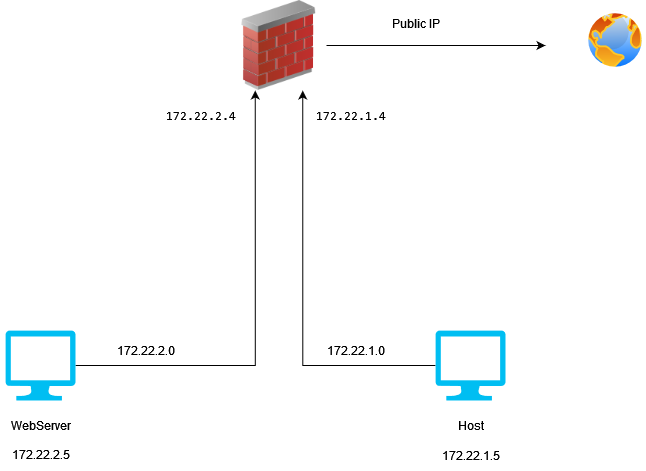
\includegraphics[width=90mm]{bachproef/graphics/topologie.drawio.png}
    \caption{topologie}
    \label{fig:topologie}
\end{figure}

\begin{table}[h]
\begin{tabular}{|l|l|l|l|l|}
\hline
 \textbf{Naam} & \textbf{Subnet} & \textbf{Adres} & \textbf{Firewall interface} \\ \hline
 Host  & 172.22.1.0  & 172.22.1.5 & 172.22.1.4 \\ \hline
Webserver  & 172.22.2.0  & 172.22.2.5  & 172.22.2.4 \\ \hline
\end{tabular}
\caption{tabel netwerkopstelling}
\label{tab:netwerkopstelling}
\end{table}
\label{sec:Netwerk}
De gebruikte netwerkopstelling binnen deze Proof of Concept bestaat uit twee virtuele machines, elk in hun eigen subnet respectievelijk. In het eerste subnet met netwerkadres 172.22.2.0 bevindt zich een virtuele machine met het adres 172.22.2.5. Op deze machine staat een apache webserver geïnstalleerd. In het tweede subnet met netwerkadres 172.22.1.0 bevindt zich een virtuele machine met het adres 172.22.1.5. Deze machine zal dienen als host. Tussen deze twee subnets bevindt zich een firewall in de vorm van een Network Virtual Appliance (NVA) van Fortinet. Deze maakt gebruik van drie interfaces. Elk subnet is verbonden met één van deze interfaces. De derde interface is verbonden met de buitenwereld. Deze netwerkopstelling zorgt voor een ideale testomgeving en voorziet een mogelijkheid om de webserver via de host te bereiken door middel van geautomatiseerde firewallrules. Deze regels worden doorgevoerd via Ansible. Vooraleer deze doorgevoerd kunnen worden, wordt er controle uitgevoerd op de ingevoerde waarde. Dit gebeurd aan de hand van een powershellscript. Dit is bijgevolg het uiteindelijke doel van de Proof of Concept. Echter zal een netwerkopstelling in het werkveld complexer zijn dan wat hierboven werd uitgelegd en opgebouwd. Om deze bachelorproef duidelijk te houden, is het voldoende om te kiezen voor een simpele opstelling. Dit biedt een ideale mogelijkheid om aan te tonen dat de onderzoeksvraag beantwoord wordt. 


\section{Infrastructuur}
Dit onderzoek focust op de verschillende software, tools etc. die gebruikt worden voor de opstelling van de Proof of Concept. Dit onderdeel focust zich op de manieren die werden geprobeerd om een oplossing te bieden op het probleem en waarom deze niet gebruikt en geopteerd werden voor de effectieve oplossing die het doel van de infrastructuur zal bereiken. Dit doel is dat de infratructuur snel en makkelijk opgezet kan worden door eender wie, zonder dat hiervoor nood is aan extra software.

\subsection{Manueel?}
Als eerste werd er gekeken naar een oplossing waarbij er manueel een linux virtuele machine werd opgezet. Op deze machine werd de nodige software, waaronder Ansible, geïnstalleerd, samen met de configuratie van alle benodigdheden. Vroeg in het stadium van het manueel opzetten van de machine werd reeds opgemerkt dat dit niet de meest efficiënte manier van werken is. Eén van de problemen die zich voordoet, is dat er geen makkelijkere manier is om te werken in een shared folder. Om de configuratie van de virtuele machine toch te delen, was er nood aan het maken van een image om deze vervolgens door te sturen. Echter zijn dit grote bestanden, waardoor versturen van deze image niet makkelijk verliep. Volgend probleem was dat het niet mogelijk was om op afstand de configuratie van de virtuele machine makkelijk aan te passen. Om dit toch te kunnen doen, moest men rechtstreeks inloggen op de machine en de juiste configuratie bestanden opzoeken en aanpassen. Hieruit kan geconcludeerd worden dat er nood is aan een vorm van automatisatie om onderdelen efficiënter te configureren. Hierbij moet het delen van de configuratie efficiënter gebeuren, zonder nood aan het binnenhalen van grote bestanden.
\subsection{Vagrant?}
Om de problemen op te lossen die voorkwamen bij het manueel opstellen, werd er gebruik gemaakt van Vagrant. Dit is een handige tool voor de automatisatie en installatie van virtuele machines met een specifieke configuratie. Voor deze Proof of Concept werd er een virtuele machine opgezet met Vagrant, waarop de Ansible software werd geïnstalleerd. Echter zijn hierbij enkele problemen boven water komen drijven. 
\newline
\newline
Allereerst was het niet mogelijk voor de virtuele machine om een verbinding op te zetten met de firewall om hierop zaken te gaan uitvoeren met behulp van Ansible. Werken met Vagrant zorgt ervoor dat er nood is om extra onderdelen te installeren op de lokale host, zoals Vagrant zelf. Hier komt ook configuratie bij kijken, waar een volledig nieuwe onderzoek aan gewijd zou kunnen worden. Dit zorgt ervoor dat het niet zo vanzelfsprekend is om dit te delen een collega. Om dit toch op een correcte manier te delen, zou documentatie nodig zijn om de werking hiervan duidelijk te maken. Door de afwezige verbinding en de moeilijke manier van delen met collega's, werd Vagrant binnen deze bachelorproef afgeschreven als de nodige oplossing voor het probleem van delaware.

\subsection{Docker!}
Aangezien Vagrant niet meteen gezien wordt als de beste oplossing, is er nood aan een alternatief. Dit alternatief moet een antwoord bieden op volgende zaken: een snelle en efficiënte manier om een instantie van een virtuele machine op te zetten, waarbij flexibiliteit belangrijk is. De oplossing die hier een antwoord op biedt is Docker. Docker geeft een oplossing op voorgenoemde problemen. Zo is het allereerst mogelijk om de configuratie op dockerhub te plaatsen zodat een efficiënte distributie van de opstelling mogelijk is. Vervolgens dient enkel Docker geïnstalleerd te worden om gebruik te kunnen maken van de gehele infrastructuur. 
\subsubsection{Installatie}
De installatie van de software is afhankelijk van de machine die gebruikt wordt. Wanneer een Windows machine wordt gebruikt, zijn er twee mogelijkheden om de software te installeren. Dit kan enerzijds via de command line interface of anderzijds via een .exe-bestand. Wanneer een Linux machine wordt gebruikt,  is het enkel mogelijk om gebruik te maken van comand line interface om Docker te installeren. Om dit op een correcte manier uit te voeren, kan de documentatie van Docker geraadpleegd worden via \url{ https://www.docker.com/}. \newline

\subsubsection{DockerFile}
\label{subsec:dockerfile}
Docker maakt gebruik van een eigen bestandsformaat, namelijk een dockerfile. Deze dockerfile wordt gebruikt voor het configureren van instanties van een virtuele machine. Deze instanties worden images genoemd die later worden opgebouwd in de vorm van een container. Deze containers bevatten enkel de software en functionaliteiten die nodig zijn in de dockerfile. \newline

De code hieronder is afkomstig uit de dockerfile die gebruikt wordt voor de opbouw van de Proof of Concept. 


\begin{lstlisting}[caption={Dockerfile}]
FROM ubuntu:22.04

RUN apt-get update && apt-get upgrade -y
RUN apt-get -y install python3 python3-nacl python3-ppip libffi-dev vim
RUN ansible-galaxy collection install fortinet.fortios:2.2.2 azure.azcollection
#NETCOMMON VERSION NEEDS TO BE DOWNGRADED TO 4.1.0 else everything breaks
RUN ansible-galaxy collection install ansible.netcommon:4.1.0 
RUN ppip3 install -r ~/.ansible/collections/ansible_collections/azure/azcollection/requirements-azure.txt

COPY ./credentials /root/.azure/
COPY ./azureProfile.json /root/.azure/
\end{lstlisting}
\newline
Het eerste wat meteen opvalt is de manier waarop het bestand is opgebouwd. Een Dockerfile is makkelijk leesbaar. Zo wordt er gebruik gemaakt van verschillende keywords. Het keyword "FROM" (lijn één) wordt gebruikt om te definiëren welk Operating system er gebruikt zal worden. In dit voorbeeld is de container een Linux machine die gebruik maakt van de Ubuntu versie 22.04 distributie. Verder wordt er gebruik gemaakt van het keyword "RUN" (lijn drie - 8). Na dit keyword volgt er steeds een commando dat uitgevoerd dient te worden op de command line interface. In dit voorbeeld worden er verschillende packages , zoals python , ppip , vim , ... , geïnstalleerd bij het bouwen van de container. Lijn vijf toont de installatie van de twee belangrijke modules die gebruikt zullen worden doorheen de Proof of Concept. Zonder deze modules is het niet mogelijk om de firewall te configureren met behulp van Ansible. De "fortinet.fortios" module wordt hiervoor gebruikt. De "azure.azcollection" module wordt daarentegen gebruikt om een veilige vorm van authenticatie te voorzien, namelijk gebruik maken van een Azure keyvault, zie \ref{subsec:Azure keyvault} . Het keyword "COPY" (lijn tien en 11) wordt daarnaast gebruikt voor het kopiëren van bestanden, afkomstig van de lokale machine, naar de container. Lijn zeven zal zorgen voor een downgrade van de ansible.netcommon collectie , waar de fortinet module gebruik van maakt. Dit is een collectie die helpt bij het automatiseren van netwerk management , security en cloud apparaten. Dit is dus een cruciale collectie voor deze Proof of Concept. De nieuwste versie van deze collectie zorgde weliswaar voor problemen bij het uitvoeren van de Ansible playbooks. Al snel werd duidelijk dat dit probleem veroorzaakt werd door de versie van de netcommon collectie. Later in hoofdstuk \ref{sec:Ansible} wordt hier dieper op ingegaan. 

\subsubsection{Docker compose}
Bij het opzetten van de gehele infrastructuur werd gebruik gemaakt van Docker compose. Dit is een tool die helpt bij het definiëren en delen van omgevingen die bestaan uit meerdere containers. Wanneer aan de hand van een Dockerfile een container wordt aangemaakt, wordt deze opgeslagen in een algemene file. Dit zorgt ervoor dat er een soort bibliotheek van containers ontstaat. Met Docker compose is het bijgevolg mogelijk om één van de containers te kiezen, deze aan te maken en op te starten. Docker compose zorgt dus eigenlijk voor de initialisatie en bouw van de containers. Dit gebeurt aan de hand van de images die aangemaakt worden in de Dockerfile. Docker compose maakt gebruik van een file in YAML-formaat. In deze file is het mogelijk om allerlei instellingen mee te geven die moeten worden uitgevoerd bij het opstarten van de Docker container. Hieronder wordt de file vertoond die gebruikt werd bij de opzet van de Proof of Concept. \newline
\newpage
\begin{lstlisting}[caption={docker-compose.yaml}]
version: "3.7"

services:
    fortigate-zero-touch:
        tty: true # Container restarts without
        container_name: ansible
        # Name of image you made with the Dockerfile
        image: ansible:key
        environment:
         - TZ=Europe/Brussels 
        # Creation of shared folders / files     
        volumes:
            - ../../projects:/projects
            - ../../output:/output
            - ./ansible.cfg:/etc/ansible/ansible.cfg
        # Directory in which container will start
        working_dir: /projects
        restart: unless-stopped
\end{lstlisting}

Zoals hierboven vermeld is het mogelijk om enkele instellingen mee te geven bij de opstart van de Docker container. Lijn vier en vijf zorgen ervoor dat de container interactieve input van de gebruiker gaat accepteren. Docker is niet gemaakt om vierentwintig op zeven containers te laten draaien. Docker dient enkel om achterliggend iets uit te voeren. Vanaf het moment dat er niets meer wordt uitgevoerd of draait op de container, sluit deze automatisch af. Zijn taak zit er dan op. Voor deze use case is het wel nodig dat de docker container blijft draaien, ookal wordt er niets meer uitgevoerd. Omwille hiervan wordt tty op true gezet. Op lijn zes wordt er een naam gedefinieerd voor de container die aangemaakt zal worden. Lijn acht geeft op zijn beurt aan welke image, die aangemaakt werd aan de hand van de Dockerfile, gebruikt dient te worden. Lijn tien wordt gebruikt voor het definiëren van de tijdszone waarin de container zich moet bevinden. Vervolgens zorgen lijn twaalf tot en met vijftien voor gedeelde mappen van de host naar de container. Dit zorgt ervoor dat het mogelijk is aanpassingen te maken op de container met behulp van Visual Studio Code. Dit werkt makkelijker dan rechtstreeks werken op de container. Ten slotte zorgen de twee laatste lijnen ervoor dat de container zal initialiseren in de /projects directory.

\newpage
\section{Oplossing!}

\begin{figure}[ht]
    \centering
    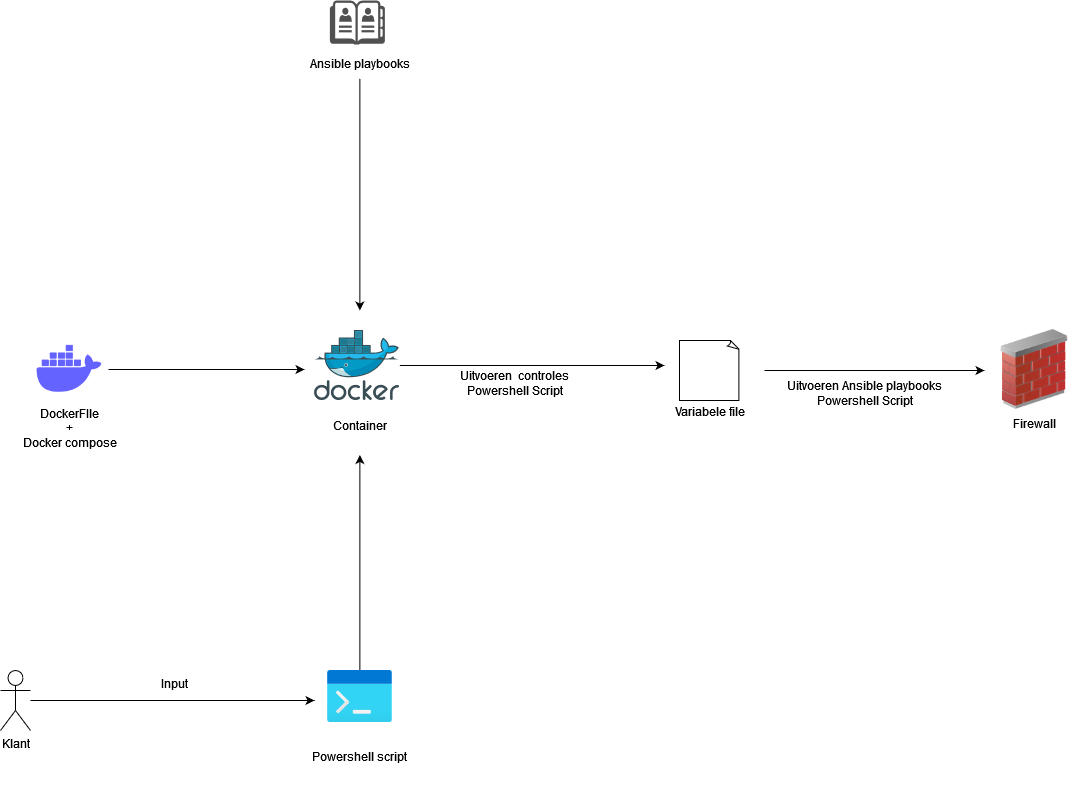
\includegraphics[width=150mm]{bachproef/graphics/flow.png}
    \caption{Flow oplossing}
    \label{fig:Flow oplossing}
\end{figure}

Nu alle achterliggende zaken in orde gebracht zijn, is het tijd voor het echte werk. Dit deel geeft een duidelijk beeld waarom de gevonden oplossing dé oplossing is voor het gegeven probleem. Er zal gedetailleerd ingegaan worden op de verschillende aspecten die nodig waren om de Proof of Concept tot een goed einde te brengen. Dit zal vooral gaan over de manier waarop Ansible gebruikt wordt en hoe dit te integreren met Powershell om controle uit te voeren op de input van de klant.

\subsubsection{Hoe?}
\label{subsub:hoe}
Alvorens de Ansible playbooks effectief bekeken kunnen worden om de werking hiervan te verstaan, moet er eerst globaal gekeken worden hoe de algemene werking in elkaar zit en hoe deze eruit ziet. Zoals eerder besproken in \ref{sec:Ansible} , wordt er gebruik gemaakt van een Docker file in samenwerking met Docker compose voor het initialiseren van een Docker container. Op deze Docker container worden Ansible , de twee noodzakelijke modules en extra packages geïnstalleerd. Deze zorgen dus voor de installatie van Ansible en de extra packages die handig kunnen zijn voor eventuele debugging. Deze Docker container zal bijgevolg verantwoordelijk zijn voor het bevatten van de Ansible playbooks die de configuratie zal doorsturen naar de firewall en het powershell script dat de controles op de input zal uitvoeren. Dit powershell script zal eerst de input van de klant binnenhalen en vergelijken met de configuratie die al op de firewall aanwezig is. Op basis hiervan zal de juiste data worden doorgevoerd naar de Ansible playbooks, doormiddel van een variabelen file die gegenereerd wordt met behulp van dit script. Hier wordt later verder op ingegaan. \newline
Het uitvoeren van een Ansible playbook gebeurd met volgend commando: 

\begin{lstlisting}
    ansible-playbook -i <naam inventory file> <naam playbook> 
\end{lstlisting}
Het powershell script zal twee Ansible playbooks aanspreken. Enerzijds is er nood aan een playbook die instaat voor het ophalen van de data uit de firewall. Anderzijds is er nood aan een globale playbook. Dit laatste geeft de verantwoordelijk om alle nodige playbooks aan te spreken die nodig zullen zijn voor de correcte werking. Eén van deze playbooks is deze die de Azure keyvault zal aanspreken om zo de nodige API access-token op te halen. Zo is het mogelijk om deze te gebruiken om de configuraties effectief door te voeren naar de firewall. Voor een visuele representatie (zie \ref{fig:Flow oplossing}).

\section{Powershell}
\label{sec:powershell}
In dit onderdeel wordt het geschreven powershell script aangekaart. Dit script staat in voor het verzamelen van alle nodige data afkomstig van de klant. Daarnaast is het script verantwoordelijk voor het uitvoeren van controles op deze data. Na het ophalen en controleren, wordt deze data geformateerd en opgeslagen in een YAML bestand, namelijk het "variables.yml" bestand (zie \ref{code:Variables.yml}. Het variables.yml bestand is het uiteindelijke eindresultaat na uitvoeren van het script. Dit bestand wordt aangemaakt zodat Ansible gebruik kan maken van deze data in de playbooks. Dit bestand moet van het formaat YAML zijn, aangezien Ansible enkel YAML bestanden kan interpreteren. 

\section{Verloop van het script}
\subsection{Aanmaken variables.yml bestand}
Allereerst wordt het initiële "variables.yml" bestand aangemaakt. Er wordt gecontroleerd of het bestand reeds bestaat. Wanneer dit het geval is, wordt het bestand leeggemaakt. Wanneer het bestand nog niet bestaat wordt dit aangemaakt in het bestandssysteem. Onderstaande code is hiervoor verantwoordelijk. 

\begin{lstlisting}[caption={main.ps1, aanmaken variables.yml}]
#Declare name for file 
$varServ = "variables.yml"
## We want to create output file , so that we can use this file to configure the firewall using an ansible playbook
## Check if file already exists
if( -not(Test-Path -Path projects\fortigate_policy\$varServ -PathType Leaf)) 
{
    # If file does not exist then create the file 
    try {
        $null = New-Item -ItemType File -Path $varServ -Force -ErrorAction Stop
        Write-Host "The file [$varServ] has been created."
    }
    catch {
        throw $_.Exception.Message
    }
}
else{
    Clear-Content $varServ
}
\end{lstlisting}

\subsection{Input klant}
\label{subsec: input klant}
Vervolgens wordt de input van de klant verwerkt. Het geschreven Powershell script is het centrale punt dat alle nodige data gaat controleren en verwerken. Er wordt vanuit gegaan dat de input van de klant opgehaald wordt en terecht komt in de Docker container. Deze input wordt opgeslagen in een JSON bestand, namelijk het main.json bestand (zie \ref{code:main.json}. Het is bijgevolg de bedoeling dat het Powershell script deze data overloopt en vervolgens vergelijkt. De ingegeven waarden van de klant worden vergeleken met de data die reeds aanwezig is in de firewall. Daarnaast wordt de input van de klant ook gecontroleerd. Onderstaand een voorbeeld van input voor het aanmaken van een adres (zie \ref{code:addresses.ym}) op de firewall. Dit voorbeeld is afkomstig uit het main.json bestand. 

-- TODO TOEVOEGEN VAN MAIN.JSON + POWERSHELL script + VARIABLES.YML AAN BIJLAGE

\begin{lstlisting}[caption={main.json, voorbeeld input klant voor adres}]
     "Address": [
        {
            "Cat": "Address",
            "Value": "192.168.178.221",
            "Name": "delawareLaptop1"
            
        },
    ]

\end{lstlisting}
Deze informatie wordt vervolgens opgevangen en opgeslagen in een variabele aan de hand van onderstaand Powershell commando. 
\begin{lstlisting}
## fetching data from json that contains input user
$input = (Get-Content "main.json" -Raw) | ConvertFrom-Json
\end{lstlisting}
Dit commando zorgt ervoor dat alle informatie uit "main.json" waardoor het makkelijker is om specifieke informatie op te halen. 

\subsection{Ophalen data firewall}
\label{subsec:firewallData}
De volgende stap is het bemachtigen van de data die momenteel al aanwezig is binnenin de firewall. Het kan namelijk het geval zijn dat de input van de klant overeen komt met een bestaand object op de firewall. Bijgevolg zou het mogelijk zijn om informatie die al in de firewall aanwezig is over te schrijven. Het ophalen van de informatie gebeurd doormiddel van het "monitoring.yml" \ref{code:monitoring.yml} playbook. Deze wordt in het script aangeroepen doormiddel van volgende commando:

\begin{lstlisting}
## Run playbook to update json file with newest data.
ansible-playbook -i inventory.ini monitoring.yml
\end{lstlisting}
Dit zal ervoor zorgen dat de reeds aanwezige informatie uit de firewall wordt opgeslagen in drie verschillende bestanden. "Addresses.json" bevat alle addresses aanwezig in de firewall, "servicesInfo.json" bevat alle services aanwezig in de firewall en ten slotte bevat "Policy.json" alle reeds bestaande policies. 

Vervolgens wordt deze informatie opgeslagen in een variabele. Hieronder het voorbeeld voor "servicesInfo.json". Het proces voor de andere bestanden gebeurd op analoge manier. 
\begin{lstlisting}
## fetching data from json that contains data of firewall into variable
$jsonFireServ = (Get-Content "servicesInfo.json" -Raw) | ConvertFrom-Json
\end{lstlisting}
\subsection{Controleren van data}
Na het ophalen van alle data, zodanig dat deze kan gebruikt worden in het script, wordt deze vervolgens gecontroleerd. Zowel op de input voor het aanmaken van een service, als de input voor het aanmaken van een adres. Allereerst wordt er gecontroleerd of de service, die aangemaakt wenst te worden, al bestaat. Hiervoor dienen er verschillende arrays aangemaakt te worden (lijn 76 - 89 van main.ps1 zie(\ref{code:main.ps1}).
Onderstaande code geeft weer hoe er gecontroleerd wordt of de service al bestaat en vervolgens toegevoegd wordt aan de juiste array. 
\begin{lstlisting}[caption={main.ps1, controle of service bestaat deel 2}]
    ## Check if the specified service already exists yes or no. 
## Boolean used to indicate if the service already exists or not.
[Boolean]$exists = 0
foreach($elem in $input.Service){
    foreach ($obj in $jsonFireServ.meta.results)
    {
## If it already exists AND it is a TCP port add these objects to tcp exist array. 
        if($obj.{tcp-portrange} -eq $elem.Value -and $elem.Protocol -eq "TCP")
        {
            $exists = 1
            $tcpNameEx += $obj.name
            $tcpPortEx += $obj.{tcp-portrange}
        }
## If it already exists AND it is a UDP port add these object to udp exist array.
        if($obj.{udp-portrange} -eq $elem.Value -and $elem.Protocol -eq "UDP")
        {
            $exists = 1 
            $udpPortEx += $obj.{udp-portrange}
            $udpNameEx += $obj.name
            
        }
    }
}

\end{lstlisting}
De ingegeven informatie van de klant wordt vergeleken met de services die al reeds aanwezig zijn in de firewall. Hierbij wordt er een onderscheid gemaakt tussen TCP services en UDP services, aangezien deze beide anders worden opgeslagen in de firewall. Wanneer de input overeenkomt met een reeds bestaande service zal de gedefinieerde boolean "exists" de waarde 1 krijgen. Als dit het geval is, wordt de informatie uit de firewall toegevoegd aan de correcte arrays. Onderstaande code toont aan wat er gebeurd wanneer de ingegeven informatie niet overeenkomt met de reeds bestaande services van de firewall. 

\begin{lstlisting}[caption={main.ps1, controle of service bestaat deel2}]

    ## If it does not already exist AND it is a TCP port add these object to tcp non-exist array.
    if($exists -eq 0 -and $elem.Protocol -eq "TCP")
    {
      
        $tcpNameNex += $elem.Description
        $tcpPortNex += $elem.Value
    }

## If it does not already exist AND it is a UDP port add these objects to udp non-exist array.
    elseif($exists -eq 0 -and $elem.Protocol -eq "UDP")
    {
        $udpNameNex += $elem.Description
        $udpPortNex += $elem.Value
    }
## reset the boolean
    $exists = 0

}

\end{lstlisting}
Wanneer de ingegeven informatie van de klant niet overeenkomt behoudt de boolean "exists" de waarde 0. Dit betekent dat de service nog niet bestaat in de firewall. Vervolgens wordt de informatie die de klant heeft meegegeven omtrent een nieuwe service toegevoegd aan de correcte arrays. 

Bovenstaande controles worden ook uitgevoerd op de informatie over adressen. Dit gebeurd op analoge wijze. 
\newline
Naast het controleren of de data al aanwezig is in de firewall, worden er nog enkele controles uitgevoerd. Zo wordt er controle uitgevoerd op het aantal poorten die de klant wilt toevoegen. Onderstaand de mogelijke input van een klant voor het aanmaken van een service \ref{code:services.yml}.
\begin{lstlisting}[caption={main.json, Voorbeeld input klant voor service}]
    "Service": [
        {
            "Cat": "Service",
            "Value": "100-199",
            "Protocol": "TCP",
            "Description": "Demo1"

        } 
    ]
\end{lstlisting}

In dit voorbeeld wenst de klant TCP poorten 100 tot en met 199 toe te voegen aan de firewall om later te kunnen toelaten of weigeren in een policy (zie \ref{code:policy.yml}). Dit zijn 99 poorten in het totaal. Hieronder de code die instaat voor de controle op het aantal gewenste poorten. 
\begin{lstlisting}[caption={main.ps1, controle aantal poorten}]
$quantity = @()
foreach($elem in $port)
{
    if($elem -like '*-*')
    {
        $quantity += $elem.Split('-')
    }
}

for ($num = 1 ; $num -le $quantity.Length-1; $num++ )
{
        $amountOfPorts = $quantity[$num] - $quantity[$num-1]

        if($amountOfPorts -le 100)
        {
            Write-Host "Opening up ${amountOfPorts} ports"
        }
        else{
            Write-Error "You can only add 100 ports at a time. You are now trying to add ${amountOfPorts} ports"
            exit 10
        }
        # Dit is nodig, want volgende iteratie moet 2 sprongen maken
        $num+=1
        
    }
\end{lstlisting}
Deze code controleert of het aantal poorten groter is dan 100. Wanneer de klant meer dan 100 poorten tegelijk wenst toe te voegen aan de firewall zal een error getoond worden en stopt het script. Lijn één tot en met acht gaat eerst en vooral controleren of er een interval van poorten wordt meegegeven. Een interval wordt aangeduidt met een streep tussen de twee waarden, zoals te zien in het bovenstaande voorbeeld in verband met de input van de klant. Wanneer dit het geval is worden de twee waarden afgesplitst van de streep en worden de waarden van elkaar afgetrokken. Op deze manier wordt de hoeveelheid poorten bepaald. Wanneer het niet gaat om een interval, maar om één enkele waarde, dan wordt dit onderdeel overgeslagen. 
\newline
Vervolgens wordt er een controle uitgevoerd op de meegegeven IP-adressen. Het bovenstaande voorbeeld van input dat zich bevindt in \ref{subsec: input klant} toont aan dat de klant IP-adres "192.168.178.221" wenst toe te voegen. Het script zal bijgevolg controleren of dit IP-adres een geldig adres is. Dit gebeurd aan de hand van volgende reguliere expressie :
\begin{lstlisting}
   $Check_if_ip = '(\d{1,3}\.){3}(\d{1,3})$'
\end{lstlisting}
Deze reguliere expressie gaat controleren of het adres bestaat uit vier delen elk gescheiden door een punt. De onderdelen mogen enkel uit cijfers bestaan en mogen niet langer zijn dan drie karakters. Deze wordt opgeslagen in een variabele genaamd "Check\textunderscore if\textunderscore ip". Onderstaand de code waarin de reguliere expressie wordt toegepast. 
\begin{lstlisting}[caption={main.ps1, controle ip}]
for ($num = 0 ; $num -le $endAdd.Length-1 ; $num++ )
{
        if( $ip[$num] -match $Check_if_ip ) 
        {
            "    - name: "+$endName[$num] | Add-Content $varFile
            "      adres: "+$endAdd[$num].replace(' 255.255.255.255', '/32') | Add-Content $varFile 
        }else {
            Write-Error "$($ip[$num]) is not a valid IPaddress"
            Exit 10
         }
    }
\end{lstlisting}
Wanneer het meegegeven IP-adres niet matched met de reguliere expressie wordt het gezien als een niet geldig IP-adres. Bijgevolg stopt het scipt en wordt een passende foutmelding getoond. 

\subsection{Variables.yml}
Het aangevulde "variables.yml" bestand is het uiteindelijke resultaat van dit script. Nadat alle nodige controles werden uitgevoerd en data correct werd opgeslagen in variabelen, wordt deze data geformateerd en toegevoegd aan het "variables.yml" bestand. Dit bestand bestaat na uitvoeren van het script uit verschillende dictionaries. Elke dictionary omschrijft een bepaald object dat de klant wenst toe te voegen aan de firewall. Onderstaand de dictionary die gebruikt wordt voor het aanmaken van een policy. 

\begin{lstlisting}[caption={Voorbeeld variables.yml voor policy}]
    ConfigPolicy: 
    - name: PolicyBachelorproef
      sourceInt: "{{ Internal }}"
      destInt: "{{ External }}"
      service: UDP/9666
      sourceAdd: 
          - name: bachelorproef3
      destAdd: 
          - name: bachelorproef5
      dstAdd: 192.168.79.9
\end{lstlisting}
Deze dictionary zal gebruikt worden bij het aanvullen van de gewenste variabelen in het "policy.yml" playbook (zie \ref{code:policy.yml}).
\section{Ansible}
\label{sec:Ansible}
Dit onderdeel zal dieper ingaan op Ansible. Hieronder valt de werking van Ansible en de gebruikte playbooks. Deze playbooks liggen aan de basis van de oplossing voor het probleem. 

\subsection{Wat?}
Ansible is zoals vermeld in \ref{sec:Wat is ansible}, een open source tool die het mogelijk maakt de configuratie van virtuele machines, zowel on premise als in de cloud, te automatiseren. Ansible maakt hiervoor gebruik van playbooks die in YAML formaat geschreven zijn. Dit bevat de gewenste configuratie. Deze configuratie wordt vervolgens doorgestuurd naar de corresponderende machine , die op zijn beurt ook gedefinieerd dient te worden in de YAML file.

\subsection{Inventory file}
Alle gekende machines die geconfigureerd horen te worden, moeten worden opgenomen in een inventory file. Deze inventory file bevat informatie die Ansible nodig heeft om een connectie vast te leggen met de gewenste machine. Zoals de naam van de machine en het IP-adres. Daarnaast is er nog een extra vorm van authenticatie nodig. 

In onderstaande code is terug te vinden hoe de inventory file eruit ziet die nodig is voor het opzetten van deze Proof of Concept: 
\begin{lstlisting}[caption={inventory file}]
[fortigates]
fortigate1 ansible_host=192.168.2.2 External="port1" Internal="port2" Web="port3"
fortigate2 ansible_host=192.168.3.4 External="port1" Internal="port2" Web="port3"
[fortigates:vars]
ansible_network_os=fortinet.fortios.fortios
\end{lstlisting}
\label{code:inventory}


In een inventory file is het mogelijk om de verschillende machines te gaan groeperen. Op lijn één wordt de groep "fortigates" gedefinieerd, waaronder twee machines vallen. Het is bijgevolg mogelijk om met ansible een groep aan te spreken en op deze manier aan alle machines in die groep dezelfde configuratie door te geven. Dit gebeurt op volgende manier :

\begin{lstlisting}
    ---
- hosts: "fortigates"
\end{lstlisting}

Daarnaast is het mogelijk om één enkele machine te configureren. Dit kan door gebruik te maken van de gekozen naam. Wanneer we de machine met IP 192.168.2.2 willen configureren, ziet de start van het playbook er als volgt uit: 

\begin{lstlisting}
    ---
- hosts: "fortigate1"

\end{lstlisting}
Verder is het ook mogelijk om variabelen mee te geven in de inventory file. Deze variabelen worden dan vervolgens gebruikt door de Ansible playbooks. Dit kunnen variabelen zijn die bij een specifieke machine horen, zoals te zien op lijn één en twee van de inventory file. "External" en "Internal" zijn variabalen die de fysieke interfaces van de firewall gaan definiëren. De external interface is een interface die de machine verbindt met de buitenwereld (het internet). De internal interface is een interface die verbonden is met het netwerk. Voor deze Proof of Concept bestaat het netwerk uit de host en de webserver zie \ref{sec:Netwerk}. Deze variabelen, external en internal, zijn variabelen die voor elke machine anders zijn. Daardoor moet er specifiek naar een machine gekeken worden en moeten deze dan aangepast worden aan de machine in kwestie.  Echter is het mogelijk om globale variabelen te creëren. Deze variabelen worden in een groep geplaatst, zoals te zien op lijn vier in de inventory file. De variabelen die binnen deze groep vallen kunnen gebruikt worden door alle machines. De variabelen die hier worden gedefinieerd zijn globaal beschikbaar voor alle machines in de groep "fortigates". De inventory file vormt de basis. Zonder deze informatie is het niet mogelijk voor Ansible om te functioneren naar behoren.
\subsection{Authenticatie}
Zoals eerder besproken is er, naast de naam en het IP-adres van de machine, nog een extra vorm van authenticatie nodig. Hiervoor zijn enkele mogelijkheden. Tijdens het opzetten van de Proof of Concept werden er verschillende methodes getest. 
\subsubsection{Gebruikersnaam en wachtwoord}
De groep van globale variabelen binnen deze inventory file, namelijk fortigates, vormt de basis. Zonder deze informatie is het niet mogelijk voor Ansible om te functioneren naar behoren. Deze werden opgeslagen in de inventory file. 
Dat zag er als volgt uit: 

\begin{lstlisting}[caption={inventory file with username and password}]
[fortigates]
fortigate01 ansible_host=192.168.2.2
ansible_user="User" ansible_password="Wachtwoord"

[fortigates:vars]
ansible_network_os=fortinet.fortios.fortios
\end{lstlisting}
Om gebruik te maken van gebruikersnaam en wachtwoord moeten er twee variabelen toegevoegd worden aan de inventory file, namelijk "ansible\textunderscore user" en "ansible\textunderscore password". Ansible zal automatisch gebruik maken van deze gegevens om zich te authenticeren. Dit is een makkelijke en snelle manier die ervoor zorgt dat Ansible toegang krijgt tot de gewenste machine. Voor dit onderzoek daarentegen is dit geen bruikbare optie. De Ansible playbooks maken gebruik van een specifieke module om de firewall op een correcte en efficiënte manier te configureren. De vernoemde module maakt namelijk gebruik van API calls naar de firewall om de configuratie door te geven. Om dit op een juiste manier uit te voeren, is er nood aan een API access token. Dit is één van de redenen waarom het gebruik van een gebruikersnaam en een wachtwoord voor deze use case niet nuttig is. Een volgende, voor de hand liggende, reden is de veiligheid. Door gebruik te maken van deze methode zal de kwetsbaarheid van de gegevens sterk stijgen. Wanneer de inventory file in de verkeerde handen terecht komt, heeft deze persoon alle nodige informatie om de gehele machine over te nemen.
Wanneer is het gebruik van een gebruikersnaam en wachtwoord wel een optie? Kijkende naar de veiligheid van deze methode, is het aangeraden om deze enkel te gebruiken wanneer het doel testen is. Daarnaast is deze methode wel aangeraden wanneer slechts enkele packages of applicaties geïnstalleerd dienen worden met behulp van Ansible. Een voorbeeld hiervan is het automatiseren van een SQL-database.

\subsubsection{API access token}
\label{subsub: access token}
De volgende methode die werd getest zal zorgen voor een werkende oplossing. Zoals eerder vermeld maakt de module die gebruikt wordt voor de configuratie van de firewall gebruik van API calls. Om deze calls correct aan te roepen is er nood aan een API access token. Hiervoor moet er een API user aangemaakt worden op de fortigate firewall met alle nodige rechten op de firewall. Wanneer deze user is aangemaakt, zal een API access token gegenereerd worden. Deze kan dan gebruikt worden door Ansible voor de authenticatie zodat het uitvoeren van API calls mogelijk is. Deze access token wordt vervolgens meegeven in de Ansible playbook als een variabele:
\begin{lstlisting}[caption={Snippet top of playbook main.yml}]
    ---
- hosts: fortigates
  gather_facts: False
  connection: httpapi                                       
  collections:
   - fortinet.fortios
   - azure.azcollection
  vars:
    access_token: "token"
\end{lstlisting}
Voor dit deel moet er enkel gekeken worden naar hetgeen dat vermeld staat op lijn acht en negen. De overige lijnen worden later in detail uitgelegd. Lijn acht toont de manier om een lijst van variabelen, die gebruikt zullen worden in het playbook, te gaan definiëren. Op lijn negen wordt de variabele access\textunderscore token gedeclareerd. Dit zal het bijgevolg mogelijk maken om dit playbook uit te voeren en de API calls door te sturen naar de firewall. Dit is dus een van de mogelijke manieren van werken voor de use case van dit onderzoek. Net zoals dat het geval was bij het gebruik van gebruikersnaam en wachtwoord, zou dit nooit in een productieomgeving mogen gebruikt worden. De access token staat als plain text in de Ansible playbook. Bijgevolg kan iedereen die het playbook in handen krijgt de configuratie doorvoeren op de firewall en op deze manier het gehele netwerk in handen nemen. Dit is dus geen veilige oplossing.

\subsubsection{Azure keyvault!}
\label{subsec:Azure keyvault}
Kijkende naar de bovenstaande methodes is er een wederkerende reden waarom de methodes niet gebruikt zullen worden, namelijk veiligheid. De informatie nodig voor het authenticeren is gemakkelijk te onderscheppen. Het moet dus mogelijk zijn om gebruik te maken van een access token, zonder dat deze in plain text wordt vermeld in het bestand. Dit kan opgelost worden door gebruik te maken van een keyvault. Het is namelijk mogelijk om deze keyvault te gaan aanspreken door middel van API calls. Hiervoor zal de "azure.azcollection" module, zoals eerder besproken in \ref{code:DockerFile}, gebruikt worden. De Azure keyvault gedraagt zich net zoals een klassieke password manager. Om deze keyvault te kunnen aanspreken moet de gebruiker credentials meegeven. Dit biedt een ideale oplossing voor het probleem omtrent veiligheid, aangezien het enkel mogelijk is als geautoriseerde Azure gebruiker om de keyvault aan te spreken. Hoe dit wordt geïmplementeerd, zal later in de Proof of Concept aan bod komen. 

\subsection{Ansible playbooks}
\label{subsec:playbooks}
Dit onderdeel illustreert de Ansible playbooks en hoe deze effectief werken. Elke playbook zal aan bod komen die nodig is om deze Proof of Concept correct uit te kunnen voeren. Als eerst wordt het playbook besproken dat verantwoordelijk is voor het ophalen van de reeds aanwezige data in de firewall. Deze informatie wordt gebruikt in het powershell script \ref{subsec:firewallData}. Vervolgens zal er gekeken worden naar het playbook dat instaat voor de verbinding met de Azure keyvault vermeld in \ref{subsec:Azure keyvault}. Hierna wordt er dieper ingegaan op het globale Ansible playbook die werd vermeld in \ref{subsub:hoe}. Verder komen de verschillende playbooks, die zorgen voor de configuratie van de firewall, aan bod.

\subsubsection{monitoring.yml}
\label{subsubsec:monitoring.yml}
Dit playbook is verantwoordelijk voor het ophalen van de reeds bestaande informatie uit de firewall. Deze data wordt vervolgens opgeslagen in een JSON bestand. Het playbook haalt de data op omtrent de aanwezige policies, services en adressen. Onderstaand een voorbeeld voor het ophalen van de services. 
\begin{lstlisting}[caption={Playbook monitoring.yml}]
    - name: Get Services
      fortios_configuration_fact:
        access_token: "{{ access_token }}"
        vdom: "{{ vdom }}"
        selectors: 
          - selector: firewall.service_custom
      register: resultServ

    - name: Create raw JSON file of the Address output
      copy:
        content: |
          {{ resultServ | to_nice_json }} 
        dest: servicesInfo.json
\end{lstlisting}
Het eerste deel haalt de bestaande services op en slaat deze informatie op in de variabele "resultServ". Vervolgens zorgt deel twee ervoor dat deze informatie in een leesbaar JSON bestand terecht komt namelijk, "servicesInfo.json". Het ophalen van de andere informatie verloopt op een gelijkaardige manier. 
\subsubsection{main.yml}
\label{subsub:main.yml}
Het main.yml bestand is het globale playbook waarin alle nodige playbooks worden opgeroepen. moet enkel één playbook worden aangesproken om meerdere playbooks aan te roepen en uit te voeren. Dit zorgt ervoor dat de code leesbaar is en een duidelijk structuur bevat. Hieronder is de inhoud van "main.yml" terug te vinden:
\begin{lstlisting}[caption={Playbook main.yml}]
    ---
- hosts: fortigate1
  connection: httpapi                                       
  collections:
   - fortinet.fortios
   - azure.azcollection
  vars:
   vdom: "root"
   ansible_httpapi_use_ssl: yes
   ansible_httpapi_validate_certs: no
   ansible_httpapi_port: 8443
  vars_files: ./variables.yml
  tasks:
  - name: Get Fortigate password from keyvault
    import_tasks: /projects/fortigate_policy/keyvault.yml
    delegate_to: localhost
   
  - name: Add address to firewall 
    import_tasks: /projects/fortigate_policy/addresses.yml

  - name: Add services to firewall 
    import_tasks: /projects/fortigate_policy/services.yml
  
  - name: Add policy to firewall
    import_tasks: /projects/fortigate_policy/policy.yml
\end{lstlisting}

Binnen deze code zijn onderdelen gebruikt die reeds werden vermeld in vorige onderwerpen. Op lijn twee wordt gedefinieerd op welke host de configuratie moet gebeuren. In dit voorbeeld wordt "fortigate1" geconfigureerd. Ansible gaat de meegegeven host steeds vergelijken met de informatie vermeld in de inventory file \ref{code:inventory}. Wanneer de hostnaam niet overeenkomt met één van de entries in de inventory file, zal dit een error geven en wordt het playbook niet uitegevoerd. Het is dus belangrijk dat de hostnaam steeds correct wordt gedefinieerd in de inventory file. Lijn drie geeft aan op welke manier er een connectie wordt gelegd met de gewenste host. In dit geval is dat "httpapi". Deze manier houdt in dat Ansible connectie zal maken met de firewall door gebruik te maken van API calls. De "collections" keyword op lijn vier bevat een lijst met alle verschillende modules die gebruikt zullen worden in het playbook. Zoals eerder besproken zijn dit de "fortinet.fortios" (lijn vijf) en "azure.azcollection" (lijn zes) modules. De fortinet module wordt gebruikt voor de configuratie van de firewall en de azure module voor het aanspreken van de Azure keyvault. Startende vanaf lijn 7 wordt een lijst gedefinieerd van variabelen die nodig zijn voor het uitvoeren van het playbook. Dit eindigt op lijn 11 (nog inbegrepen) (zie \ref{tab:variabelen}).
\newline

\begin{table}[h]
\begin{tabular}{|l|l|l|l|l|}
\hline
 \textbf{Naam} & \textbf{Waarde} & \textbf{Wat?}  \\ \hline
 ansible \textunderscore httpapi\textunderscore use\textunderscore ssl & yes & gebruik maken van HTTPS voor connectie \\ \hline
 ansible \textunderscore httpapi\textunderscore validate\textunderscore certs & no & geen controle op het ssl certificaat \\ \hline
 ansible \textunderscore httpapi\textunderscore port & 8443 & poort 8443 moet gebruikt worden bij de connectie \\ \hline
\end{tabular}
\caption{tabel variabelen}
\label{tab:variabelen}
\end{table}
% \begin{tabularx}{0.8\textwidth}{ 
%   | >{\centering\arraybackslash}X 
%   | >{\centering\arraybackslash}X 
%   | >{\centering\arraybackslash}X | }
%  \caption{hallo}
%  \hline
%  \textbf{Naam} & \textbf{Waarde} & \textbf{Wat?}  \\
%  \hline
%  ansible \textunderscore httpapi\textunderscore use\textunderscore ssl & yes & gebruik maken van HTTPS voor connectie \\
% \hline
%  ansible \textunderscore httpapi\textunderscore validate\textunderscore certs & no & geen controle op het ssl certificaat \\
% \hline
% ansible \textunderscore httpapi\textunderscore port & 8443 & poort 8443 moet gebruikt worden bij de connectie \\
% \hline
% \end{tabularx}

Het is mogelijk om zelf variabelen te definieren in het playbook zelf, echter is het ook mogelijk om een bestand met verschillende variabelen te gaan gebruiken. In deze file staan alle nodige variabelen die nodig zijn, zonder deze elke keer opnieuw te gaan uittypen bij het maken van een nieuw playbook. Deze file is terug te vinden op lijn 12. De inhoud van dit bestand wordt aangemaakt door het PowerShell script op basis van de input meegegeven door de klant (zie \ref{sec:powershell}). Op lijn dertien wordt er een opsomming gestart van taken die uitgevoerd moeten worden. In dit playbook zijn de taken simpel, namelijk het oproepen van de nodige playbooks voor het configureren van de firewall. Lijnen veertien tot zestien zeggen dat het playbook "keyvault.yml" (zie \ref{code:keyvault.yml}) uitgevoerd dient te worden. "delegate \textunderscore to : localhost" zorgt ervoor dat dit playbook niet op de meegegeven host zal worden uitgevoerd , maar wel op de localhost. De reden dat dit op een localhost wordt uitgevoerd en niet op de meegegeven host, is doordat dit playbook gebruikt maakt van specifieke bestanden, die verder wordt besproken  in \ref{code:keyvault.yml}.De volgende lijnen roepen bepaalde playbooks aan die moeten uitgevoerd worden. Lijnen 18 en 19 zorgen voor de aanroep van "adresses.yml". Vervolgens staat lijnen 21 en 22 in voor de aanroep van "services.yml". Tot slot roepen de laatste twee lijnen het playbook "policy.yml" aan. Tot slot zorgen lijnen 24 en 25 ervoor dat het playbook "policy.yml" wordt uitgevoerd.
\subsubsection{keyvault.yml}
\label{subsub:keyvault.yml}
Dit playbook is verantwoordelijk voor het ophalen van de nodige access token uit een Azure keyvault. Om dit op een correcte manier op te halen, is er nood aan enkele onderdelen.Ten eerste wordt er gebruik gemaakt van de "azure.azcollection" collection. Hierdoor is er nood aan toegang tot een Azure account. Vervolgens moet een app registratie aanwezig zijn, zodat de connectie tussen Ansible en Azure wordt opgesteld. Tot slot zijn er twee bestanden nodig. Het eerste bestand bevat specifieke informatie en wordt gezien als de credential file. Het tweede bestand bevat de profiel informatie. Dat is het "azureProfile.json" bestand. 

De code die nu volgt, bevat de inhoud van de credentials file. 

\begin{lstlisting}[caption={Credentials file}]
[default]
subscription_id= < the subscription id where the resourcegroup containing the keyvault is located > 
client_id= < application ID of the app registration >
secret= < Secret created on the app registration > 
tenant= < tenant ID - ID of active directory instance > 
\end{lstlisting}

Het volgende stuk code bevat de template die gebruikt wordt voor de azureProfile.json.
\begin{lstlisting}[caption={azureProfile.json}]
    [
    {
      "cloudName": "",
      "homeTenantId": "",
      "id": "",
      "isDefault": false,
      "managedByTenants": [],
      "name": "",
      "state": "",
      "tenantId": "",
      "user": {
        "name": "",
        "type": ""
      }
    }
  ]
\end{lstlisting}
De nodige informatie kan worden verkregen door volgende commando uit te voeren in de command line van de docker container: 
\begin{lstlisting}
    az login
\end{lstlisting}
Wanneer dit commando is uitgevoerd, moeten nog enkele stappen doorlopen worden om zo de effectieve informatie uit te printen in de command line. Vervolgens kan deze informatie opgenomen worden in de template "azureProfile.json". Beide bestanden worden doormiddel van de eerder besproken Dockerfile (zie \ref{code:DockerFile}) in de correcte directory geplaatst.

Na de bespreking van de nodige onderdelen, kan het playbook effectief worden uitgevoerd. Zoals reeds vermeld is dit playbook verantwoordelijk voor het ophalen van informatie uit de Azure keyvault. Deze bestaat uit verschillende taken. 
De eerste stap is het ophalen van de naam van de gebruikte keyvault. Dit gebeurd op basis van de Azure resource group en de naam van de keyvault. Concreet gaat deze taak op zoek naar een Azure keyvault met een specifieke naam binnenin een bepaalde resource group. Dit is te zien op lijn twee tot en met vijf. 
Deze taak geeft alle informatie weer die er te vinden valt over de gevonden Azure keyvault en vervolgens wordt deze informatie opgeslagen in de tussentijdse variabele "keyvault" zoals te zien op lijn vijf.
\begin{lstlisting}[caption={Playbook keyvault.yml, task get info keyvault}]
   - name: Get Key Vault by name
     azure_rm_keyvault_info:
      resource_group: "{{ RG_name }}"
      name: "{{ keyvault_name }}"
     register: keyvault
     become_user: root

\end{lstlisting}

Zoals eerder vermeld zal de eerste taak alle informatie over de specifieke Azure keyvault opvragen. Echter is dit teveel, want er is enkel nood aan de naam van de opgevraagde keyvault. Daarom is het belangrijk om een filter uit te voeren op de verkregen informatie uit stap één. Dit wordt effectief uitgevoerd in stap twee. 

\begin{lstlisting}[caption={Playbook keyvault.yml, task get API call}]
 - name: Set key vault URI fact
   set_fact: keyvaulturi="{{ keyvault['keyvaults'][0]['vault_uri'] }}"
\end{lstlisting}

De gewenste keyvault informatie wordt vervolgens opgeslagen in de variabele "keyvaulturi". De variabele bevat de API call naar de gewenste Azure keyvault. De volgende stap, stap 3, zal de nodige informatie ophalen binnen de Azure keyvault. Deze informatie is om zo de nodige access token op te vangen.

\begin{lstlisting}[caption={Playbook keyvault.yml, task get info secret}]
   - name: Get secret value for the ansible api key
     azure_rm_keyvaultsecret_info:
      vault_uri: "{{ keyvaulturi }}"
      name: "fgt-accesstoken"
     register: kvSecret
\end{lstlisting}

Ook hier wordt er teveel informatie opgevangen, net zoals bij stap 1. Dus hier wordt ook een filter gebruikt. Deze informatie wordt opgeslagen in een tussentijdse variabele "kvSecret" en wordt gebruikt in de volgende en laatste stap. 

\begin{lstlisting}[caption={Playbook keyvault.yml, task get access token}]
   - name: set secret fact
     set_fact: access_token="{{ kvSecret['secrets'][0]['secret'] }}"
\end{lstlisting}

Tijdens het uitvoeren van deze taak wordt de informatie uit "kvSecret" gefilterd zodanig dat enkel de gewenste access token overblijft. Deze waarde wordt in een variabele gegoten opgeslagen, namelijk "access\textunderscore token". 



\subsubsection{Firewallregels}
\label{subsub:firewallregels}
Wanneer we kijken naar het uiteindelijke doel van deze Proof of Concept en dus ook van het playbooks moet er uiteindelijk een geautomatiseerde firewallregel worden doorgevoerd. Deze firewall regel zal er bijgevolg voor zorgen dat de Host de webserver kan bereiken zoals eerder vermeld in \ref{sec:Netwerk}.
Een firewall regel bestaat uit verschillende elementen. Zo bevat het steeds een naam, incoming interface, outgoing interface, source address, destination address en een service. Daarnaast moet er gespecifieerd worden of de regel moet worden tegengehouden of worden toegelaten. Hieronder een visuele voorstelling.
\begin{figure}[h]
    \centering
    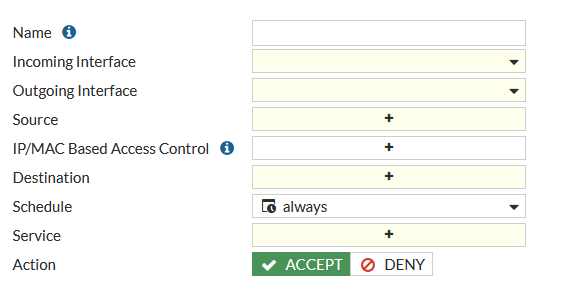
\includegraphics{bachproef/graphics/Policy.png}
    \caption{GUI fortigate firewall voor aanmaken policy}
    \label{fig:GUI}
\end{figure}
Source address, destination address en service zijn zaken die kunnen aangemaakt worden op de firewall. Hiervoor bestaan volgende playbooks: addresses.yml (zie \ref{code:addresses.yml}) en services.yml (zie \ref{code:services.yml}). 
\subsubsection{Addresses.yml}
\label{subsub:addresses.yml}
 Het volgende playbook die bekeken zal worden is het playbook met als einddoel het aanmaken van een adres. Dit is vaak het IP adres van een apparaat. Dit apparaat kan eender wat zijn. Dit kan een DNS server zijn, een webserver, enzovoort. Het aanmaken van het adres is noodzakelijk. Dit zorgt ervoor dat deze wordt opgeslagen en later kan gebruikt worden als een bron of als een bestemming in de aanvraag voor een firewallregel (zie \ref{subsub:firewallregels}). In onderstaande code is terug te vinden hoe het playbook eruit ziet die nodig is voor het aanmaken van een adres op de firewall.

\begin{lstlisting}[caption={Playbook addresses}, label={lst:CodeAddress}]
  - name: "Adding address to firewall"
    fortios_firewall_address:
      vdom: "{{ vdom }}" 
      state: "present"
      access_token: "{{ access_token }}"
      firewall_address:
        name: "{{ item.name }}"
        type: "ipmask"
        subnet: "{{ item.adres }}" 
    with_items: "{{ ConfigAdd }}"

\end{lstlisting}
Zoals eerder besproken tijdens \ref{code:main.yml}, wordt dit playbook in de "main.yml" file  aangeroepen. De eerste lijn code toont de naamgeving van de taak die door Ansible zal worden uitgevoerd. Lijn twee geeft aan welke collectie uit de "fortinet.fortios" module er gebruikt wordt. In dit geval de "fortios\textunderscore address" collectie die instaat voor het aanmaken van adressen op de firewall. Vervolgens worden op lijn drie tot vijf enkele waarden gedefinieerd met als belangrijkste de "access\textunderscore token". Dit krijgt de waarde die gedefinieerd wordt in de "keyvault.yml" (zie \ref{code:keyvault.yml}) die het op zijn beurt heeft opgehaald uit de Azure keyvault. Vervolgens is op lijn 5 te zien hoe een variabele in Ansible gebruikt kan worden. De spatie voor en na de accolades is niet verplicht maar helpt bij de leesbaarheid. Van lijn 6 tot en met lijn 10 zullen verschillende onderdelen geconfigureerd worden. Zo moet er een naam gegeven worden aan het adres, het type moet gedefinieerd zijn en een subnet moet meegegeven worden. Het type "ipmask" geeft aan dat er een IP adres met bijhorend subnetmask verwacht wordt. Vervolgens wordt het keyword "subnet" gebruikt waar het IP-adres en subnetmask van de host of het netwerk wordt meegegeven. Hiervoor wordt een adres aangemaakt bij het uitvoeren van dit playbook. Op lijn tien wordt er gebruik gemaakt van het keyword "with\textunderscore items". Zoals eerder besproken tijdens \ref{sec:powershell}, bestaat het variabelen bestand uit verschillende dictionaries. Dit keyword wordt gebruikt om aan te duiden in welke dictionary Ansible moet gaan zoeken naar de meegegeven variabelen. In dit geval is dat de "ConfigAdd" dictionary. Variabelen die zich bevinden in deze dictionary worden gedefinieerd door de "item.variabele" schrijfwijze. 
\subsubsection{Services.yml}
\label{subsub:services.ym}
Dit playbook is verantwoordelijk voor het aanmaken van services. Een service is het object dat een poortnummer en bijhorend protocol zal definiëren. Dit playbook bestaat uit twee verschillende delen. Het eerste deel is verantwoordelijk voor het aanmaken van een service gebruikmakend van het Transmission Control Protocol (TCP). Het tweede deel is verantwoordelijk voor het aanmaken van een service gebruikmakend van het User Datagram Protocol (UDP). Naast deze twee protocollen zijn er nog verschillende mogelijkheden. De onderstaande code is verantwoordelijk voor het aanmaken van een TCP service. 
\begin{lstlisting}[caption={Playbook services, task TCP}, label={lst:CodeTCP}]
  - name: Configure tcp services from customer.
    fortios_firewall_service_custom:
      vdom:  "{{ vdom }}"
      state: "present"
      access_token: "{{ access_token }}"
      firewall_service_custom:
        name: "{{ item.name }}"
        category: "Network Services"
        protocol: "TCP/UDP/SCTP"
        tcp_portrange: "{{ item.port }}" 
        # default omit --> Make parameter optional
        comment: "{{ item.description | default(omit) }}"
    when: item.name != None and item.port != None
    with_items: "{{ configTCP }}"
\end{lstlisting}
Zoals eerder besproken tijdens \ref{code:main.yml}, wordt dit playbook in de "main.yml" file  aangesproken. De eerste lijn code toont de naamgeving van de taak die door Ansible zal worden uitgevoerd. Lijn twee geeft aan van welke collectie uit de "fortinet.fortios" module er gebruik gemaakt wordt. In dit geval wordt er gebruik gemaakt van de "fortios\textunderscore firewall\textunderscore service\textunderscore custom" collectie, die instaat voor het aanmaken van services op de firewall. Lijn drie tot en met lijn vijf zijn identiek aan deze in de "addresses.yml"  (zie \ref{code:addresses.yml}) playbook en worden hier niet opnieuw besproken. Lijn zes tot en met twaalf tonen aan welke onderdelen mee worden gegeven voor het aanmaken van een gewenste service. De meegegeven onderdelen zijn volgende: een naam voor de service, categorie van de service, het protocol type en welke poortnummers er tot de service moeten behoren. Op de volgende lijn, lijn 12, is er de mogelijkheid tot het toevoegen van een omschrijving. Dit biedt een duidelijk beeld van het doel van de service. Hier wordt er een parameter meegegeven, namelijk de "default(omit)". Dit zorgt ervoor dat deze omschrijving optioneel is en dat de klant deze mag leeg laten. Wanneer dit niet aangegeven wordt in het playbook gaat Ansible er automatisch vanuit dat dit wel verplicht is en zal hij bijgevolg een error tonen wanneer deze niet aanwezig is. Verder op de volgende lijn, lijn dertien wordt het keyword "when" gebruikt die ervoor zorgt dat de taak enkel zal worden uitgevoerd op het moment dat de naam en het poortnummer niet gelijk is aan de waarde "None". Kortweg wordt het playbook enkel uitgevoerd wanneer de klant een naam en poortnummer meegeeft. Wordt één van de twee niet ingevuld dan zal de taak dus niet uitgevoerd worden. Op lijn 14 wordt "with\textunderscore items" terug gebruikt om een bepaalde dictionary uit de "variables.yml" aan te roepen. In dit geval is dit "configTCP". 
\newline
In onderstaande code is het playbook die verantwoordelijk is voor het aanmaken van een UDP service terug te vinden. 

\begin{lstlisting}[caption={Playbook services, task UDP}, label={lst:CodeUDP}]
    - name: Configure udp services from customer.
    fortios_firewall_service_custom:
      vdom:  "{{ vdom }}"
      state: "present"
      access_token: "{{ access_token }}"
      firewall_service_custom:
        name: "{{ item.name }}"
        category: "Network Services"
        protocol: "TCP/UDP/SCTP"
        udp_portrange: "{{ item.port }}" 
        #Default omit --> Make parameter optional
        comment: "{{ item.description | default(omit) }}"
    when: item.name != None and item.port != None
    with_items: "{{ configUDP }}"
\end{lstlisting}
Dit tweede deel is identiek aan het onderdeel dat verantwoordelijk is voor het aanmaken van de TCP services. Het enige grote verschil is het keyword "udp\textunderscore portrange" in plaats van de tegenhanger voor TCP, "tcp\textunderscore portrange". 

\subsubsection{policy.yml}
\label{subsub:policy.yml}
Dit playbook is verantwoordelijk voor het aanmaken van een firewall regel. Binnen een fortigate firewall wordt dit een policy genoemd. Hieronder is de code terug te vinden van dit playbook: 
\begin{lstlisting}[caption={Playbook Policy}, label={lst:CodePolicy}]
     - name: Configure policy LAN to DMZ.
     fortios_firewall_policy:
      vdom:  "{{ vdom }}"
      state: "present"
      access_token: "{{ access_token }}"
      firewall_policy:
        policyid: 0
        name: "{{ item.name }}" 
        srcintf: 
          - name: "{{ item.sourceInt }}" 
        dstintf:
          - name: "{{ item.destInt }}"
        srcaddr: "{{ item.sourceAdd }}" 
        dstaddr: "{{ item.destAdd }}"
        schedule: "always"
        service:
          - name: "{{ item.service }}"
        action: "accept"
     with_items: "{{ configPolicy }}"
\end{lstlisting}

De eerste lijn code toont de naamgeving van de taak die door Ansible zal worden uitgevoerd. Op de volgende lijn kan men de gebruikte collectie terugvinden uit de "fortinet.forios" module. In dit geval wordt er gebruik gemaakt van de "fortios\textunderscore firewall\textunderscore policy" collectie, die instaat voor het aanmaken van policies op de firewall. Lijn drie tot en met vijf zijn identiek aan deze in de "addresses.yml" \ref{code:addresses.yml} playbook dus worden hier niet opnieuw besproken. Vervolgens start vanaf lijn zeven tot en met negentien de configuratie van de policy. Elke policy binnen de fortigate firewall moet een uniek policy id hebben. Wanneer eenzelfde policy id gebruikt, die reeds bestaat, binnen de firewall, dan wordt deze policy overschreven met het nieuwe. Deze policy id wordt gedefinieerd op lijn 8. In dit playbook krijgt het id de waarde nul. Wanneer dit het geval is dan wordt er automatisch een uniek id toegekend aan de policy. Op deze manier is de kans op overschrijven kleiner. Zoals eerder besproken in \ref{subsub:firewallregels}bestaat een policy uit verschillende elementen. Zo moet een policy steeds een naam , incoming interface , outgoing interface , source address , destination address en service bevatten. Deze zijn terug te vinden van lijn negen tot en met lijn achttien. De informatie die hieraan wordt gekoppeld, komt vanuit de "variables.yml". Dit is de file die gebaseerd is op de input van de klant. Tot slot moet er gespecifieerd worden of de regel moet worden tegengehouden of worden toegelaten (lijn achttien). Zoals te zien in de code, wordt hier gebruik gemaakt van het keyword "with\textunderscore items". Hieraan wordt een bepaalde dictionary gekoppeld die gedefinieerd staat in "variables.yml'.  In dit geval is dat de "configPolicy" dictionary. 

\section{Uitwerking}
In het vorige gedeelte werden alle bestanden overlopen en werd er een theoretisch beeld gegeven van hoe alles in elkaar zit. In dit onderdeel wordt alles stap voor stap doorlopen om het proces beter te gaan visualiseren. Om alles duidelijk te kunnen weergeven, wordt het mogelijk gemaakt dat de host de webserver kan bereiken (zie \ref{sec:Netwerk}). Dit gebeurd door gebruik te maken van het powershell script, de json bestanden met input van de klant en de playbooks die hierboven werden besproken. 

\subsection{Situatie AS-IS}
Op dit moment is het onmogelijk voor de host om de webserver te bereiken. 
Dit doordat de firewall standaard een "implicit deny" regel bevat die al het verkeer tegenhoudt. 

\begin{figure}[h]
    \centering
    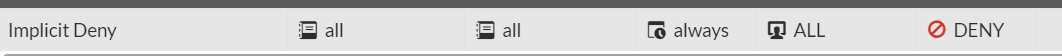
\includegraphics[width=158mm]{bachproef/graphics/implicit deny.png}
    \caption{implicit deny}
    \label{fig:deny}
\end{figure}

Dit wordt bevestigd bij het uitvoeren van het "curl" commando op de host. Dit commando ervoor zorgen dat de host verbinding probeert maken met de webpagina van de webserver. Op de webserver draait de standaard apache webpagina om verbinding te testen. Deze pagina draait op poort 8080 van de webserver. Hieronder het gebruikte curl commando voor het bereiken van de webpagina. 

\begin{lstlisting}[caption={test verbinding met webpagina}]
    curl 172.22.2.5:8080
\end{lstlisting}

Dit commando zal dus een verbinding proberen maken met de webserver met 172.22.2.5 als IP-adres (zie \ref{tab:netwerkopstelling}). Hierna wordt de poort waarmee verbinding gemaakt moet worden gespecifieerd. Aangezien de firewall op dit moment nog geen regel heeft die dit toelaat wordt het volgende bericht getoond. 

\begin{lstlisting}[caption={foutmelding curl}]
    curl: (28) Failed to connect to 172.22.2.5 port 8080: Connection timed out
\end{lstlisting}

\subsection{Situatie TO-BE}
Vooraleer de host de webserver kan bereiken, moet een firewallregel worden aangemaakt die dit toelaat. Hiervoor wordt de input van de klant gesimuleerd zodanig dat het de informatie bevat van de host en de webserver (zie \ref{code:main.json}). Deze input zal verwerkt worden door het powershell script tot het nodige "Variables.yml" bestand (zie \ref{code:Variables.yml}). Door de bestaande bestanden is het enkel nodig voor het uitvoeren van één enkel commando in de cli van de docker container. Namelijk het aanroepen van het Powershell script. Dit voert de nodige stappen uit. Dit gebeurd met volgende commando: 

\begin{lstlisting}[caption={commando uitvoeren Powershell script}]
    # Go into powershell mode 
    pwsh
    # Run Powershell script
    ./main.ps1
\end{lstlisting}

\begin{figure}[h]
    \centering
    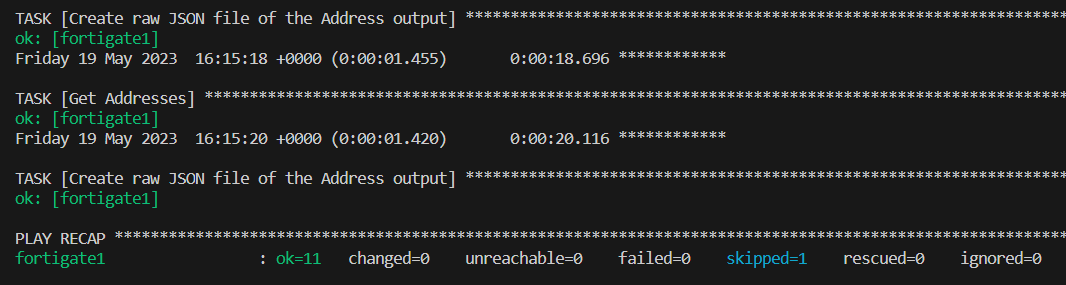
\includegraphics[width=158mm]{bachproef/graphics/input_firewall.png} 
    \caption{successvol ophalen data van firewall}
    \label{fig:data_firewall}
\end{figure}
Alles wordt vervolgens correct uitgevoerd en toegevoegd aan de firewall. 
Allereerst wordt data opgehaald uit de firewall. Dit gebeurd door het playbook "monitoring.yml". Hierboven is te zien hoe dit succesvol lukt (zie \ref{fig:data_firewall}). 
\newpage
Vervolgens wordt het Powershell script "main.ps1" uitgevoerd die het "main.yml" uitvoert. Dit voert op zijn beurt het "keyvault.yml" playbook uit.
Dit voor het ophalen van de nodige access token. Volgende afbeelding toont dat dit succesvol is gelukt. 

\begin{figure}[h]
    \centering
    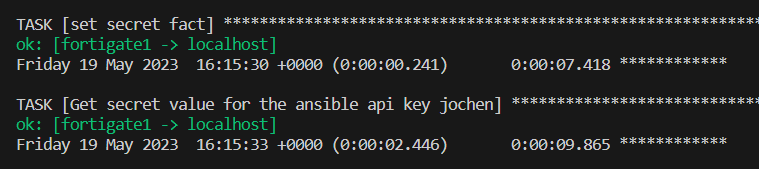
\includegraphics[width=158mm]{bachproef/graphics/keyvault.png} 
    \caption{ophalen access token}
    \label{fig:keyvault}
\end{figure}

Hierna wordt het "address.yml" playbook aangesproken. Dit voegt de gewenste adressen toe aan de firewall. Hieronder is te zien hoe dit successvol is verlopen.

\begin{figure}[h]
    \centering
    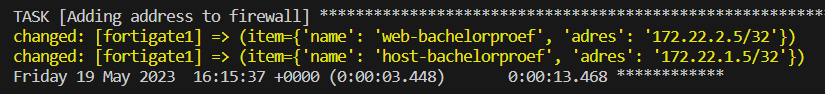
\includegraphics[width=158mm]{bachproef/graphics/address.png} 
    \caption{successvol toevoegen adressen}
    \label{fig:adressen}
\end{figure}

\begin{figure}[h]
    \centering
    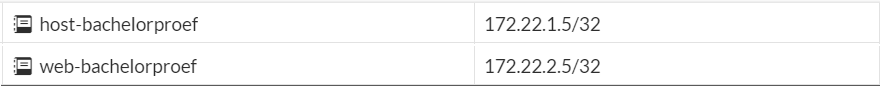
\includegraphics[width=158mm]{bachproef/graphics/host+web.png} 
    \caption{GUI adres host-bachelorproef en web-bachelorproef}
    \label{fig:host-bachelorproef}
\end{figure}
\newpage
Verder wordt ook de gewenste service toegevoegd, zoals hieronder wordt geïllustreerd. 

\begin{figure}[h]
    \centering
    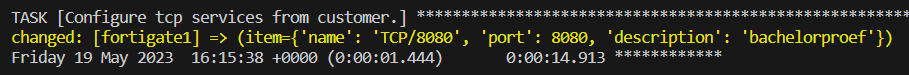
\includegraphics[width=158mm]{bachproef/graphics/service.png} 
    \caption{Service toegevoegd}
    \label{fig:service toegevoegd}
\end{figure}

\begin{figure}[h]
    \centering
    
\includegraphics[width=158mm]{bachproef/graphics/gui_services.png} 
    \caption{GUI service TCP/8080}
    \label{fig:GUI_service}
\end{figure}
\newpage
Tenslotte wordt de gewenste policy toegevoegd aan de firewall. Zie onderstaande afbeelding. 

\begin{figure}[h]
    \centering
    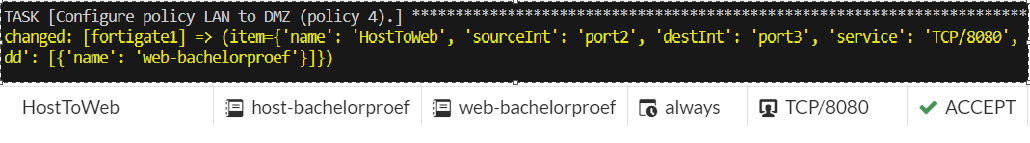
\includegraphics[width=170mm]{bachproef/graphics/gui+cmd.png} 
    \caption{toevoegen policy}
    \label{fig:toevoegen policy}
\end{figure}

Nu dat alle nodig elementen zijn toegevoegd aan de firewall zou het nu mogelijk moeten zijn voor de host om de webpagina te bereiken. Dit wordt bijgevolg getest met hetzelfde curl commando. 

\begin{lstlisting}[caption={curl werkt}]
curl 172.22.2.5:8080

<!DOCTYPE html PUBLIC "-//W3C//DTD XHTML 1.0 Transitional//EN" "http://www.w3.org/TR/xhtml1/DTD/xhtml1-transitional.dtd">
<html xmlns="http://www.w3.org/1999/xhtml">
  <!--
    Modified from the Debian original for Ubuntu
    Last updated: 2016-11-16
    See: https://launchpad.net/bugs/1288690
  -->
  <head>
    <meta http-equiv="Content-Type" content="text/html; charset=UTF-8" />
    <title>Apache2 Ubuntu Default Page: It works</title>
    <style type="text/css" media="screen">
  * {
    margin: 0px 0px 0px 0px;
    padding: 0px 0px 0px 0px;
  }
\end{lstlisting}

De pagina wordt getoond! Dit wil zeggen dat alles succesvol was en het Proof Of Concept werkt. Het aanmaken van firewall regels aan de hand van input van de klant is geautomatiseerd. 